% Source for the figure of mergeSort() on 1, 7, 4, 6, 2, 8, 3, 5 (sec. 12.3,
% exercise 11.1 of Morin's book): the parts after each level of merges.
% Build: make figures (in ../build).
\documentclass[border=4pt]{standalone}
\usepackage[T1]{fontenc}
\usepackage{lmodern}
\usepackage{amsmath,amssymb}
\usepackage{tikz}
\usepackage{lamalunga}
% tikz-ads.tex: the TikZ styles shared by the figures of the memory of the
% manual, \input by each standalone figure: a cell of a vector (cell), the
% cell that an operation touches (touched), a free cell (free), a node of a
% linked structure (node), the labels of indices (index) and of variables
% (var), a pointer (ptr), and \cells and \indices to draw a row of cells.
\usetikzlibrary{arrows.meta,positioning,calc,fit,shapes.multipart}
\definecolor{adsTouched}{RGB}{214,196,236}
\definecolor{adsFree}{RGB}{236,236,236}
\tikzset{
  ads/.style={>={Stealth[length=2mm]},font=\small,
              every node/.append style={inner sep=0pt}},
  cell/.style={draw,minimum width=7mm,minimum height=7mm,
               font=\small\ttfamily,outer sep=0pt},
  touched/.style={cell,fill=adsTouched},
  free/.style={cell,fill=adsFree,text=black!45},
  node/.style={draw,rounded corners=1pt,minimum width=8mm,
               minimum height=6mm,font=\small\ttfamily},
  index/.style={font=\scriptsize\ttfamily,text=black!60},
  var/.style={font=\small\itshape},
  ptr/.style={->,thick}
}
% \cells{name}{x,y}{list}: a row of cells, the first at (x,y), named
% name-0, name-1, ...; each item is text/style, the style one of cell,
% touched and free (e.g., {a/cell,e/touched,/free})
\newcommand{\cells}[3]{%
  \foreach \v/\s [count=\i from 0] in {#3}
    \node[\s] (#1-\i) at ($(#2)+(\i*7mm,0)$) {\v};}
% \indices{name}{n}: the indices 0 .. n-1 under the cells of name
\newcommand{\indices}[2]{%
  \foreach \i in {0,...,\numexpr#2-1\relax}
    \node[index,below=1.2mm of #1-\i] {\i};}

\begin{document}
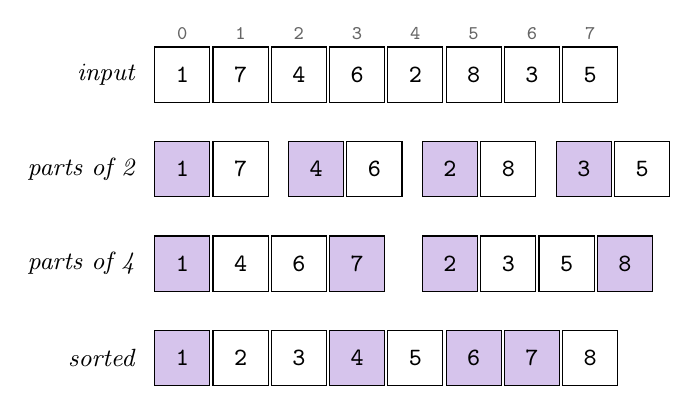
\begin{tikzpicture}[ads]
  % \row{y}{label}{x offsets as list of value/style}
  \newcommand{\grp}[3]{\foreach \v/\s [count=\i from 0] in {#3}
     \node[\s] at ($(#1)+(\i*7.4mm,0)$) {\v};}
  \node[var,anchor=east] at (-6mm,0) {input};
  \grp{0,0}{}{1/cell,7/cell,4/cell,6/cell,2/cell,8/cell,3/cell,5/cell}
  \node[var,anchor=east] at (-6mm,-12mm) {parts of 2};
  \grp{0,-12mm}{}{1/touched,7/cell}
  \grp{17mm,-12mm}{}{4/touched,6/cell}
  \grp{34mm,-12mm}{}{2/touched,8/cell}
  \grp{51mm,-12mm}{}{3/touched,5/cell}
  \node[var,anchor=east] at (-6mm,-24mm) {parts of 4};
  \grp{0,-24mm}{}{1/touched,4/cell,6/cell,7/touched}
  \grp{34mm,-24mm}{}{2/touched,3/cell,5/cell,8/touched}
  \node[var,anchor=east] at (-6mm,-36mm) {sorted};
  \grp{0,-36mm}{}{1/touched,2/cell,3/cell,4/touched,5/cell,6/touched,7/touched,8/cell}
  \foreach \i in {0,...,7} \node[index] at (\i*7.4mm,5.2mm) {\i};
\end{tikzpicture}
\end{document}
